\chapter{基于全局的特征提取算法}

\section{基本框架}
PCA\cite{turk1991face}是近代人脸识别中较早的方法.在文献中,作者于1991年评价了之前基于人脸手工的标定,专家模型构建的方法,并且指出了人工方法的若干不足之处.同时提出了基于统计的PCA方法,成功实现了自动的人脸识别系统.并且,作者提出了\textit{eigenface}这个用来表征人脸图像投影的空间.从那以后,研究者们从多个角度研究了许多除了\textit{eigenface}以外的方法,提出了\textit{fisherface}\cite{kwak2005face}等一系列特征空间.

这些基于统计的方法都有着不同的出发点,但在实现上都是比较相似的.他们从不同的角度来尝试从人脸数据库中分解出更有代表性的分量,并把那些分量作为特征空间的基底.当处理新入样本时,新的样本和创建的特征空间基底作投影操作,得到的样本坐标就是该样本在空间的表示.以下是本文中所尝试的方法及其主要思想:
\begin{center}
  \footnotesize
        \captionof{table}{本文中所尝试的降维方法及其主要思想}
  \begin{tabular}{l|c}
  \hline 
    方法 & 主要思想 \\ \hline
    PCA & 在假设样本高斯分布的情况下,寻找样本空间特征值最大的k个正交向量作为基底\\ \hline
    NMF & 由于图片仅由正实数表示,提出了保证特征向量也为正数的前提下的特征分解方法\\ \hline
    ICA & 在假设样本独立统计(I.I.D)及非高斯分布的情况下,来近似估计各个独立分量成分\\
    \hline
  \end{tabular}
\end{center}
\subsection{人脸分解的例子}
下面以PCA为例,来表示一个具体的基于全局的人脸特征提取算法的工作流程.
\paragraph{构建基底空间} 这一步骤是不同方法的主要区分之处,不同的算法主要是从不同的角度来构建更为优化的投影空间,使得投影后的样本坐标更具有表现力.
\newline
下面是通过分解ORL数据库所有图片得到的前6张特征脸(\textit{eigenfaces})和平均脸:

\begin{center}
\begin{minipage}[t]{\linewidth}
%\label{fig:main}
\center
{
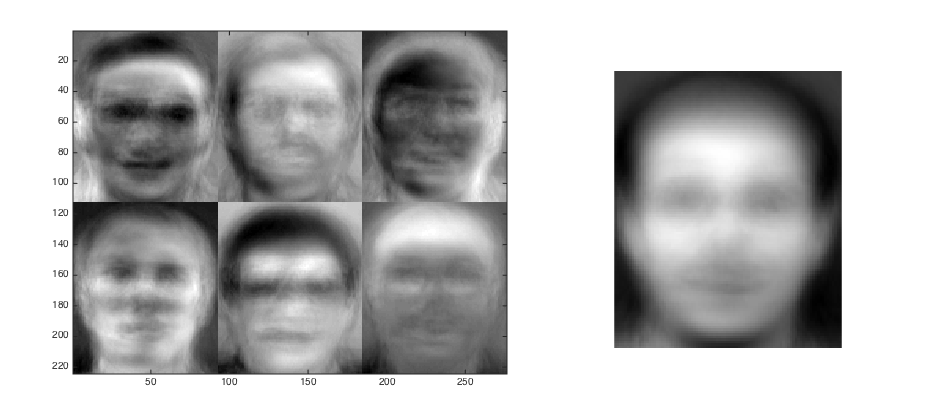
\includegraphics[width=\MyFactor\textwidth]{Img/pca_eigenspace.png} \captionof{figure}{前6张特征脸和平均脸}
}
\end{minipage}
\medskip
\end{center}

其中,PCA的计算在给出特征向量的同时,还会给出代表特征向量权重的特征值,上述6个特征值在400个特征向量空间中占据了51.4\%的权重.权重分布如下图:

\begin{figure}[!htbp]
\centering 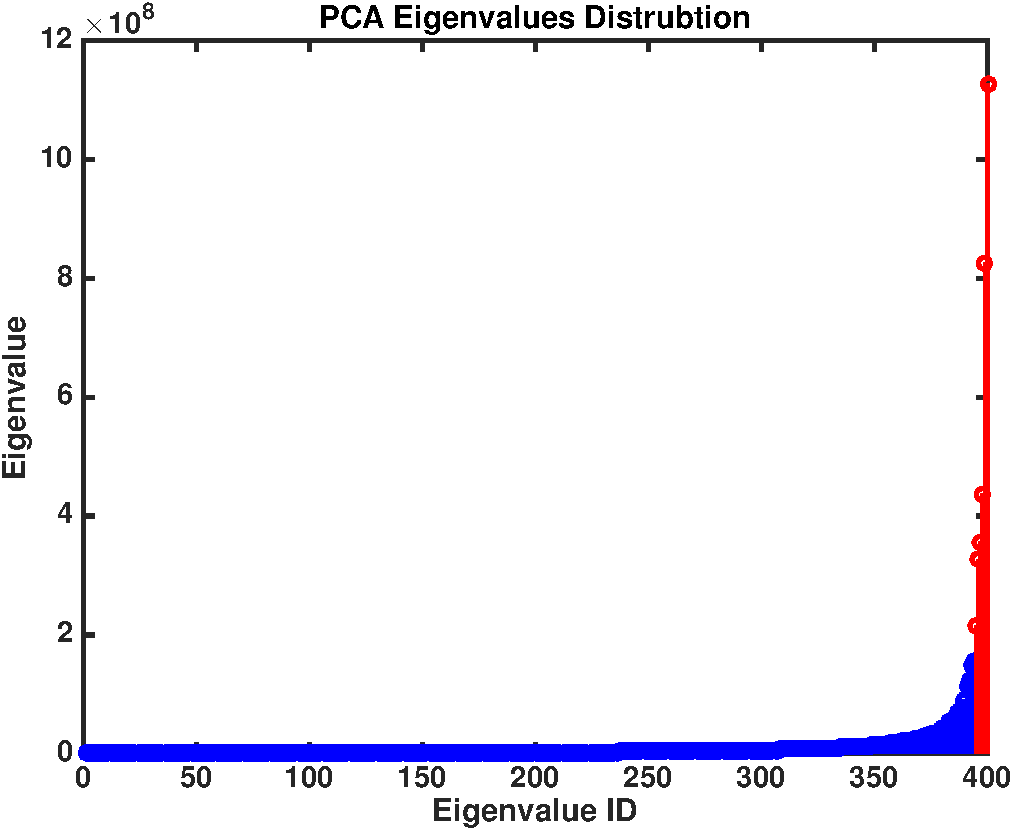
\includegraphics[width=\MyFactor\textwidth]{Img/pca_eivalue.pdf} 
\caption{特征值分布图 \\ 蓝色:舍弃的特征向量, 红色: 保留的特征向量}
\end{figure}
设特征向量组成的基底矩阵为V, 输入图像为I, 则该步骤可以表示为:
\begin{equation}
Weights = Inv(V) \cdot I
\end{equation}
其中
\begin{itemize}
	\item V为一个$m  \times  n$的矩阵,m是特征脸的像素数,n是特征向量的数目,$Inv(V)$为其转置矩阵
	\item I为一个$m \times d$的矩阵,m是特征脸的像素数,d是需要分解的输入图像数目
	\item Weights为一个$n \times d$的矩阵,n是特征向量的数目,d是需要分解的输入图像
\end{itemize}


本例中图像在特征向量空间下的权值如下:
\begin{center}\begin{tabular}{|l|l|l|l|l|l|}
\hline
-123.7915&-689.9194&261.7842&1867.0258&1072.1813&1531.176\\\hline
\end{tabular}
\end{center}

\paragraph{输入样本重构} 这一步是根据上一步求得的权值来线性地重构这张输入样本.当然了,当实际应用时不需要恢复原始输入图片时,这一步可以省略.

\begin{center}
\begin{minipage}[t]{\linewidth}
%\label{fig:main}
\center
{
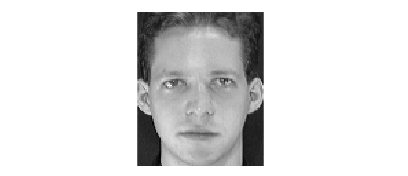
\includegraphics[width=\MyFactor\textwidth]{Img/pca_sample.png} \captionof{figure}{左:输入图像 右:重建后的图像}
}
\end{minipage}
\medskip
\end{center}

	
	以下是该流程的简要示意:
\begin{center}
\begin{minipage}[t]{\linewidth}
%\label{fig:main}
\center
{
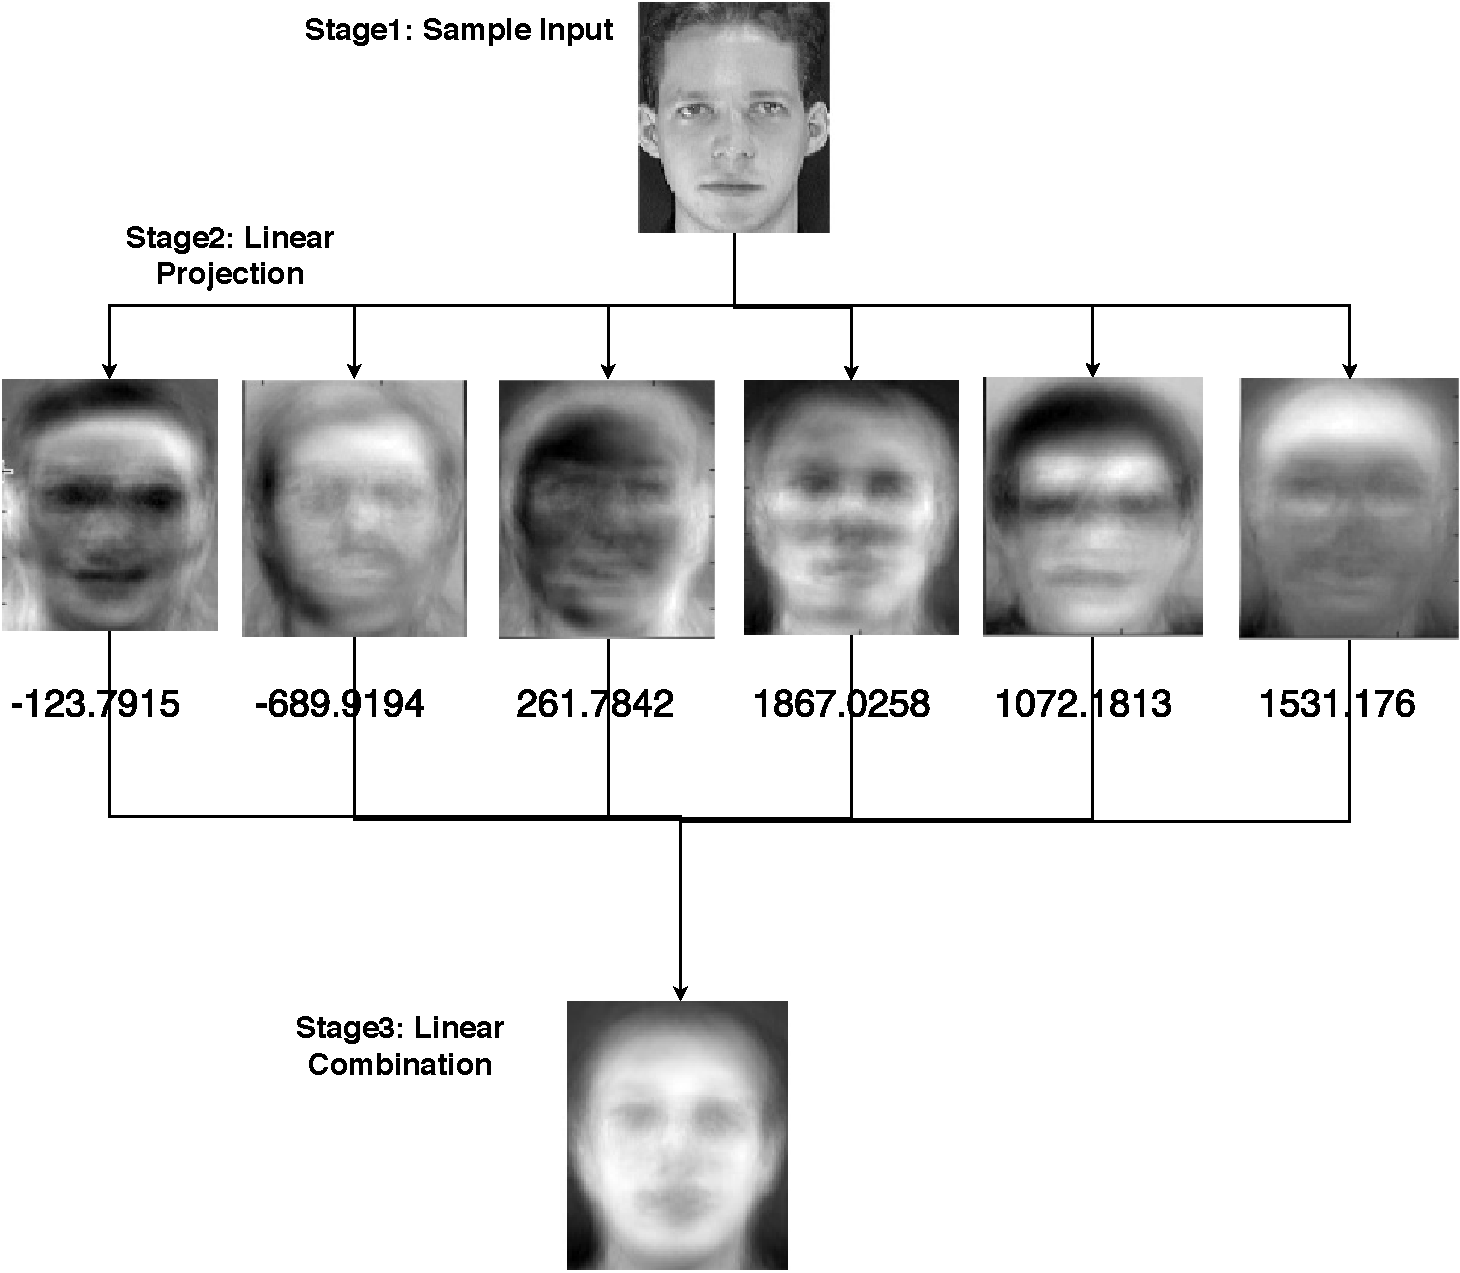
\includegraphics[width=\MyFactor\textwidth]{Img/pca_demo.pdf} 
\captionof{figure}{图像投影示意}
}
\end{minipage}
\medskip
\end{center}

\subsection{两类不同的特征空间}
\label{sec:arch2}
\begin{center}
\begin{minipage}[t]{\linewidth}
%\label{fig:main}
\center
{
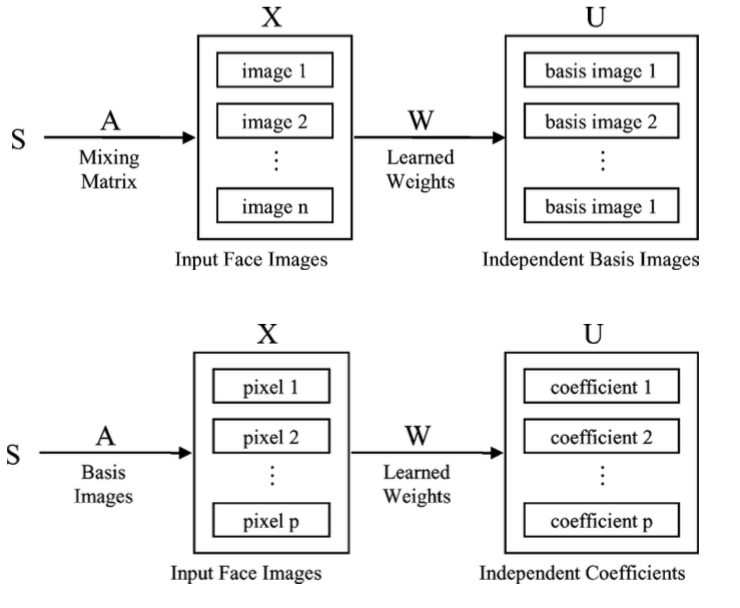
\includegraphics[scale=1]{Img/ica_c1c2.png} 
\captionof{figure}{图像投影示意 \\ 上: Architecture I, 下: Architecture II. 来源\cite{draper2003recognizing}}
}
\end{minipage}
\medskip
\end{center}
值得指出的是,受到\cite{draper2003recognizing}启发.这里同时存在着两类不同的分解思想.他们的区别在于一类的输入样本是另一类的转置.\\



第一类的思想是将人脸图像作为变量而将每张图像上的像素作为这个变量的描述,而分解的操作发生在人脸的空间上.


第二类的思想是将人脸图像样本作为各个像素的描述,并且转而把像素作为变量.
\\
在实践中由于第二类的维数过高,运算量太大,采用了第一类.

\section{PCA}
本章节的主要依据文献是\cite{turk1991eigenfaces, turk1991face},从本章节开始,将依次简要介绍PCA, NMF, ICA的基本原理和计算方法.并在ORL数据库下给出其特征脸空间. \newline

根据\cite{de2010face, smith2002tutorial},当PCA的运算数据中减去其平均值(又称为平均脸),PCA运算等价于KL运算.所以本文也是对KL运算的介绍.\newline

\subsection{PCA的思想}
\begin{enumerate}
	\item 记$\tau_i$为由第i张基底计算集图像形成的图像.原始图像是一个$m \times n$大小的矩阵,$\tau$为一个原始图像按照行展开形成的$ m \times n$长的行向量
	\item 记\begin{equation}\Phi = \frac{1}{M}\Sigma_{n-1}^M\tau_n\end{equation}$\Phi$是$\tau_i$的平均值,也就是这个基底计算集的平均脸,M是基底计算集的样本数目
	\item 记\begin{equation} \label{Centering} \phi_i = \tau_i - \Phi\end{equation}
	\item PCA旨在选择值最大的若干$\lambda$,\begin{equation} \lambda_k = \frac{1}{M}\Sigma^M_{n=1}(u^T_k \phi_i)^2\end{equation} 同时,$u_k$受到正交性的限制:\begin{equation}\label{pca:corr} u_k \times u_l = \left\{\begin{array}{c}
        1(k = l)\\
        0(k \neq l)
    \end{array}\right.
    \end{equation}其中$\lambda$被称作特征值,$u$被称作特征向量,也就是所求的特征基底.
	\item $\lambda_k$的个数是需要选择的,选择的特征向量数越多,保留的内容就越多,但同时压缩效果就越差
\end{enumerate}
\subsection{PCA的计算方法}
从线性代数的角度,PCA相当于最小化这个样本集的二阶统计值,当PCA完成后,各个特征向量之间的相关性为0.而$u$,$\lambda$分别为相关矩阵C的特征值,特征向量.
\begin{equation}
	C = A \cdot A^T
\end{equation}
A是样本集,也就是$[\phi_1, \phi_2,...,\phi_M]$\\ 

由于C为一个$(m \times n) \times (m \times n)$大小的矩阵,直接计算不便,经分析,对C的计算等价于对L的计算,L定义为
\begin{equation}
	L = A^T \cdot A
\end{equation}
L是一个$M \times M$大小的矩阵.
而计算过程也就是计算L矩阵的特征向量,特征值.而此时的特征向量$v$并非直接可用的向量,其大小为$M \times M$,而选择过k个特征值最大的的向量后,其大小为$M \times k$,需要使用计算
	\begin{equation}
		u=A \cdot v
	\end{equation} 
	便得到了大小为$(m \times n) \times k$的特征基底.
	
\subsection{PCA的在ORL测试集的投影基底}
以下是使用ORL数据集400张图片作为基底,选择特征值最大的前64张图片得到的特征基底.
\begin{center}
\begin{minipage}[t]{\linewidth}
%\label{fig:main}
\center
{
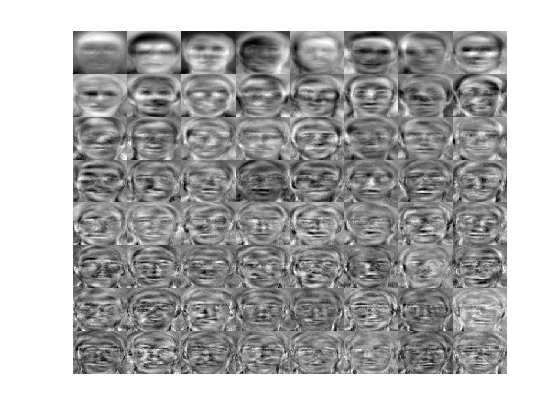
\includegraphics[width=\textwidth]{Img/pca_base.png} \captionof{figure}{PCA的在ORL测试集的投影基底}
}
\end{minipage}
\medskip
\end{center}

同时需要注意的是,PCA所得到的基底是特征向量,而特征向量之间由\ref{pca:corr}满足正交性,所以特征向量$Basis = [u_1,u_2,...,u_k]$构成的矩阵是正交矩阵,满足$Basis' = Basis^T$. 为了说明这一点,以下是上述基底两两之间的相关距离根据\ref{pca:corr}计算得到的距离矩阵:
\begin{center}
\begin{minipage}[t]{\linewidth}
%\label{fig:main}
\center
{
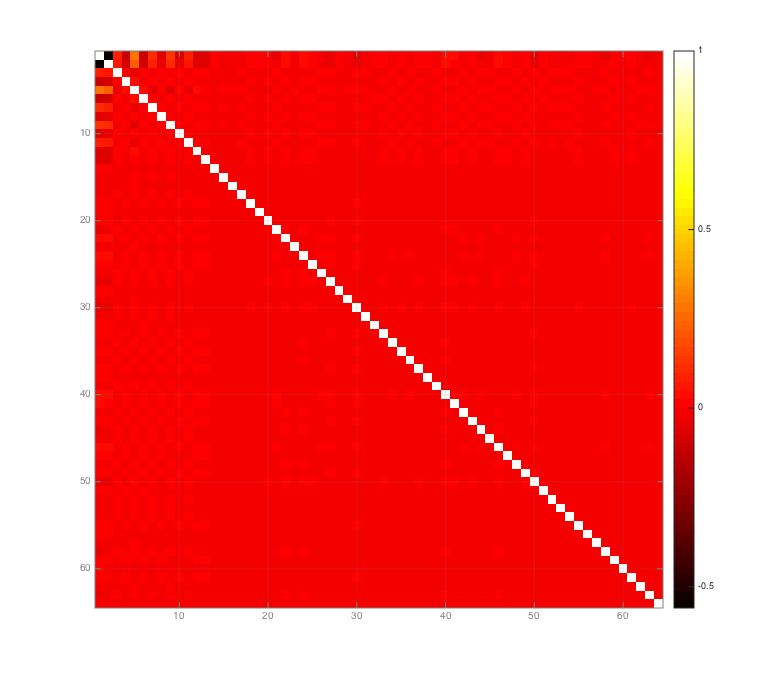
\includegraphics[width=\MyFactor\textwidth]{Img/pca_correlation.png} \captionof{figure}{PCA基底的正交性}
}
\end{minipage}
\medskip
\end{center}
由上图可见,大部分基底之间的相关性均接近于0.

\section{NMF}

\subsection{NMF的思想和计算方法}
本章节的内容主要基于\cite{lee1999learning, lee2001algorithms}.\newline

NMF算法围绕着在保证分量非负性的同时达到$V=W \cdot H$的分解.
	其中
	\begin{enumerate}
		\item V与等价于上一章节的$[\tau_1, \tau_2,...\tau_M]$,是基底计算样本的全集.
		\item W为一个$(m \times n) \times k$的矩阵
		\item H为一个$k \times m$的矩阵.可以由此得到$W \cdot H$是一个$(m \times n) \times M$的矩阵,和V有相同的形状.
	\end{enumerate}
 NMF定义了惩罚函数\begin{equation}
 \label{nmf_cost} ||V-W\cdot H|| = \Sigma_{ij} = (V_{ij} - WH_{ij})^2\end{equation}来描述分解的效果.$||V-W\cdot H||$是V和WH之间的欧式距离.实现完全分解时$||V-W\cdot H||=0$

NMF算法提出了保证W,H非负性的前提下的迭代公式,并证明了其收敛性,使用迭代的方法来逐步逼近最终的W,H.其迭代公式如下
	\begin{equation}
		\label{equ: nmf_iter1}
		H_{au} = H_{au}\frac{(W^TV)_{au}}{(W^TWH)_{au}}
	\end{equation}
	\begin{equation}
		\label{equ: nmf_iter2}
		W_{ia} = W_{ia}\frac{(VH^T)_{ia}}{(WHH^T)_{ia}}	
	\end{equation}
可以看到H,W的迭代运算中使用的仅仅是除法,乘法和加法,而同时V矩阵初值均为正数这就保证了H,W的非负性.

完成迭代后,舍弃H,认为W矩阵就是这个数据集的非负分解结果,也就是这个数据集的特征向量基底.\newline

同时,需要注意的是
\begin{itemize}
	\item 上述的迭代公式并非全局最优解.对于$||V-W\cdot H||$这个优化函数,目前并没有可以同时优化W和H的方法.NMF方法采用的是迭代的方法,也就是,优化H时,以上一步的W为目前最佳W,优化W时,以上一步的H为目前最佳H.而其该局限性使得这种优化方法只能收敛到局部最小值,并且每次结果都和初始值有关.\cite{berry2007algorithms}.
	\item 上述的迭代公式,惩罚函数只是NMF思想的一种实现方式.现实中还有其他的替代方法.在\cite{lee1999learning, lee2001algorithms}就列写了另一个惩罚函数和对应的迭代公式,还有对应迭代公式收敛性的证明.其惩罚函数为$$\Sigma_{ij}A_{ij} log \frac{A_{ij}}{B_{ij}} - A_{ij} + B_{ij}$$
\end{itemize}

\subsection{NMF的终止条件}
在\cite{lee1999learning, lee2001algorithms}中,并没有对NMF算法的终止条件作出说明,而NMF算法的终止条件也有很多种不同的解释,由于实际计算中很难达到理想的$V=WH$的条件,因此需要在算法收敛速度较慢时提前终止算法.
\begin{itemize}
	\item 在\cite{hoyer2004non}的算法中,其NMF算法是一个无限循环,而需要用户根据W和H的分解情况来自行中断程序.
	\item 在\cite{brunet2004metagenes}中,其NMF算法根据分析结果是否不再变化达到稳定而中断程序.
\end{itemize} 

本文的方法采用和\cite{brunet2004metagenes}类似的方法,这是一种经验方法,矩阵C的构建仅仅是为了描述结果的结构.具体来说,它的工作方法是:
	\begin{enumerate}
		\item 首先对于H矩阵(其形状为$k \times m$),得到每栏k个元素中最大值的位置,其取值从1到k,共计有m个
		\item 对这m个元素构成的向量Vect,构建对称布尔矩阵C,其中$C_{ij}$和$C_{ji}$为真代表Vect向量中第i个元素的位置和第j个元素的值相同.这在H矩阵中,代表的含义是第i列列向量中最大值的位置和第j列列向量中最大值的位置一样
		\item 迭代时,比较C和之前结果,如果差别比较小(本项目中为小于15个元素的差别),则认为迭代已经进入了稳定
		\item 当连续若干次C都和上一次迭代有近似相同结果时(本项目中设定连续6次),则终止程序
	\end{enumerate}

以下是使用该方法后某次的运行结果,
\begin{enumerate}
	\item 第一栏为迭代次数,每10次输出一次.
	\item 第二栏为满足稳定性条件后迭代次数的计数,当某次迭代使计算结果不再和之前相同时,该变量会被刷新.
	\item 第三栏为和上一次迭代比较不同结果的C元素个数计数,当满足小于15个元素和上一次计算结果不同时,开始第二栏的计数.
\end{enumerate}

\begin{multicols}{4}
\begin{verbatim}
	10	0	378
	20	0	506
	30	0	352
	40	0	344
	50	0	186
	60	0	196
	70	0	62
	80	0	86
	90	0	44
	100	0	34
	110	0	26
	120	0	30
	130	0	30
	140	0	32
	150	1	10
	160	0	24
	170	0	18
	180	0	28
	190	1	6
	200	2	10
	210	0	40
	220	1	0
	230	2	2
	240	3	12
	250	4	12
	260	0	24
	270	1	8
	280	2	14
	290	3	4
	300	4	0
	310	5	4
	320	6	0
	\end{verbatim}
\end{multicols}
以下是对应的迭代过程中惩罚函数\ref{nmf_cost}下降曲线的绘制,所计算的输入量是120个,需要求得64个特征向量
\begin{center}
\begin{minipage}[t]{\linewidth}
%\label{fig:main}
\center
{
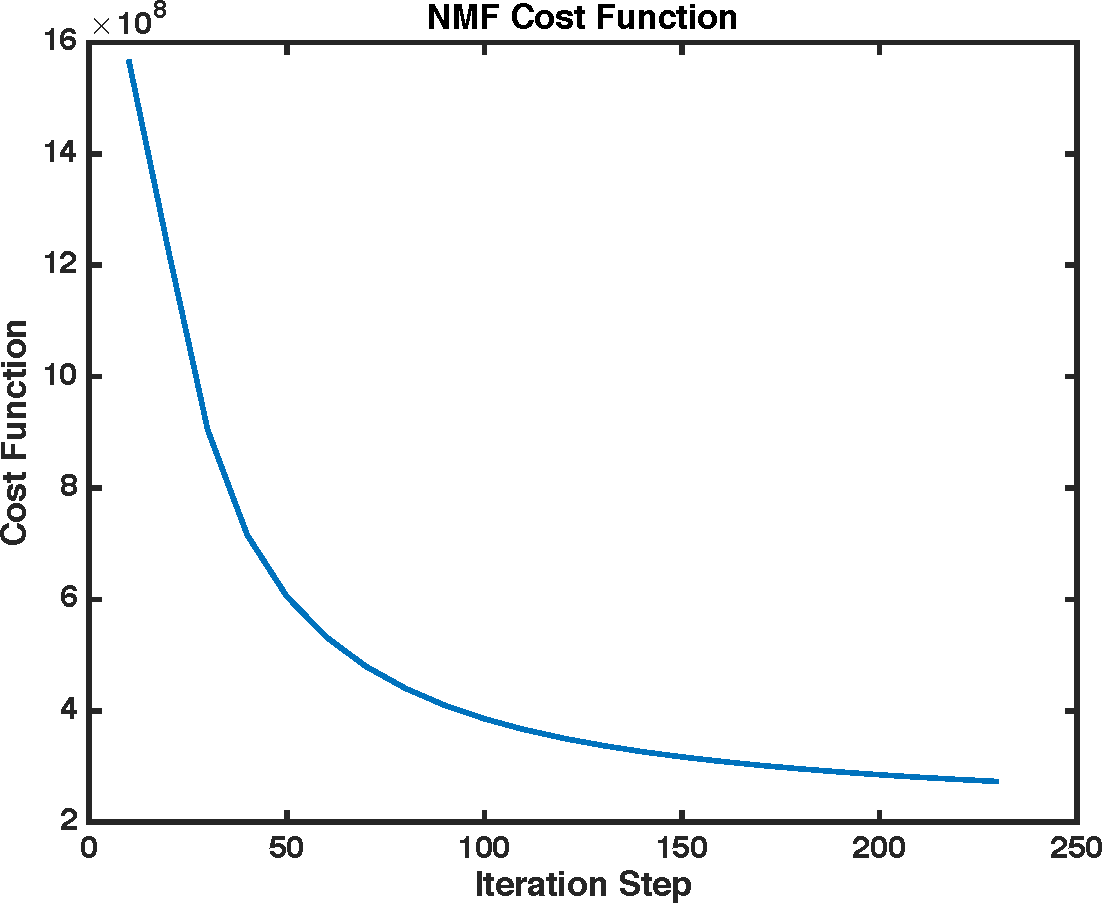
\includegraphics[width=\MyFactor\textwidth]{Img/nmf_cost.pdf} \captionof{figure}{NMF的惩罚函数下降曲线 \\ x坐标:迭代次数, y坐标 惩罚函数\ref{nmf_cost}}
}
\end{minipage}
\medskip
\end{center}

\subsection{NMF的在ORL测试集的投影基底}
以下是使用ORL数据集120张图片作为基底(40个人,每人三张),选择结果的前64张图片得到的特征基底.只选择120个图片用来计算是因为NMF的计算速度较慢.
\begin{center}
\begin{minipage}[t]{\linewidth}
%\label{fig:main}
\center
{
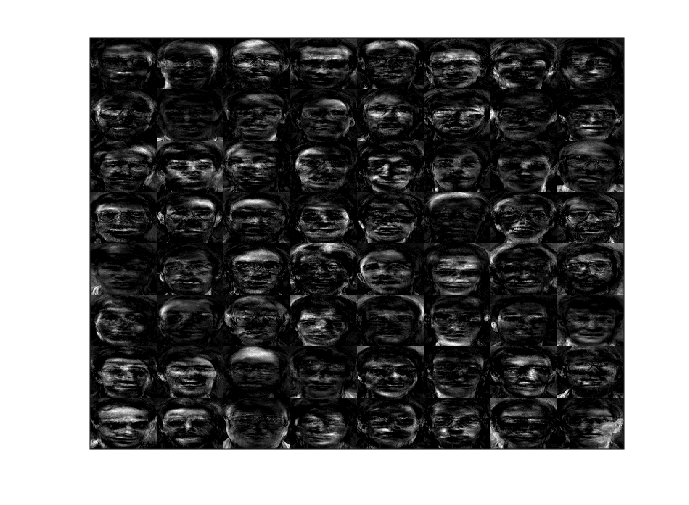
\includegraphics[width=\textwidth]{Img/nmf_base.png} \captionof{figure}{NMF的在ORL测试集的投影基底}
}
\end{minipage}
\medskip
\end{center}


由于NMF基底不是正交的,使用了\textit{Matlab}函数中\textit{Pinv()}函数计算了伪逆来投影.
\section{ICA}
\subsection{ICA的思想和计算方法}
ICA被有些文献称为PCA的延伸,对于PCA,它使得样本之间的二阶统计量最小化,对于ICA,它使得样本中二阶及以上的统计量最小化,也就是使得样本之间独立.所谓的独立性,指的是 \begin{equation}
		f_s(s) = \prod_i f_{s_i}(s_i)
	\end{equation}
	其中$f_s$是信号的分布密度函数.

本章节所主要依据的文献是\cite{icafordummies, draper2003recognizing, vaseghi2006principal, langlois2010introduction, hyvarinen2000independent, awasthyanalysis, khaparde2008fastica}\newline

ICA试图解决如下问题:\begin{equation}
	x = As
\end{equation}
其中,已知的只有混合后的信号x,A为混合信号时的权值,s为信号源.ICA试图在未知A的情况下求得s.

为了进一步简化问题,ICA作出如下假设,假设x的长度与s的长度一致.也就是,混合信号的数量和信号源的数量一致.这使得A成为一个方阵.同时,也使得A可逆,记其逆矩阵为W.那么有下列关系:
\begin{equation}
	\label{ICA:SourceDecompose}
	s=Wx
\end{equation}
ICA的核心就是在估计W来更好的得到s.\newline

ICA的推导中对变量有一定的要求,需要进行一些预处理,这些操作有:
\begin{enumerate}
	\item{中心化} 该步使用公式\ref{Centering},使得$ \tau_i$平均值为0
	\item{白化} 该操作使得各个变量之间无关(uncorrelated)并且方差为1.也就是满足\ref{pca:corr}.该步操作可以在输入样本上执行PCA来完成.
\end{enumerate}
如此可见,PCA处理过的结果满足ICA的要求,因此PCA常常被用来ICA的预处理操作.PCA处理过的结果不仅满足ICA的预处理要求,并且PCA预先对样本进行了降维操作,简化了ICA的运算.\newline

白化后,开始按照\label{ICA:SourceDecompose}来进行分解.目前共有两类不同思想的ICA实现方法,分别是\textit{FastICA}和\textit{InfoMax}.下面进行简要介绍.
	\paragraph{FastICA}	\textit{FastICA}使用\textit{Negentropy}来表征变量间的独立程度,\textit{Negentropy}的定义为
	\begin{equation}
		J(y) = H(ygauss) - H(y)
	\end{equation}
	J是一个非负数,表征了参数的非高斯性,当为0时,为高斯分布.
	
	可使用\textit{Kurtosis}来近似\textit{Negentropy},\textit{Kurtosis}公式为
	\begin{equation}
		kurt(y) = E(y^4) - 3(E(y^2))^2
	\end{equation}
	E(y)代表y的期望值(下同)
	
	近似后的结果为
	\begin{equation}
		J(y) \approx \frac{1}{12}E(y^3)^2+\frac{1}{48}kurt(y)^2
	\end{equation}
	并可被进一步近似为
	\begin{equation}
		J(y) \approx \Sigma^p_{i=1}k_i[E(G_i(y)) - E(G_i(v))^2]
	\end{equation}
	当仅仅使用一个函数G时,可进一步近似为
	\begin{equation}
	\label{ica_g}
		J(y) \propto (E(G(y)) - E(G(v)))^2
	\end{equation}
	
	G是可以被定义的,\cite{hyvarinen2000independent}中给出了比较有用的形式:
	\begin{multicols}{2}
		\begin{equation}
			G_1(u) = \frac{1}{a_1}log(cosh(a_1u))
		\end{equation}
	
		\begin{equation}
			G_2(u) = -exp(-u^2/2)
		\end{equation}
	\end{multicols}
	其中的$a_1$是常数, $1 \leqslant a_1 \leqslant 2$.\newline


	而\textit{FastICA}算法就是一种类似牛顿法的使用梯度下降法(Gradient Descent)方法来逼近J最大值的方法. 
	
	\paragraph{InfoMax}
	\textit{FastICA}从信息论的角度,来求得最大的\textit{Negentropy},而\textit{InfoMax}则从最小化\textit{Mutual information}的角度出发.
	
	\textit{Mutual information}的定义是
	\begin{equation}
		I(y_1,y_2,...,y_m) = \Sigma_{i=1}^m H(y_i) - H(y)
	\end{equation}
	\cite{hyvarinen2000independent}中,推导得到,经过ICA预处理过程的变量,满足\begin{equation}
			I(y_1,y_2,...,y_m) = C - \Sigma_iJ(y_i)
		\end{equation}
		其中C是一个常数.
		
		由此可见,I和J是相关的变量.而\textit{FastICA}中J的最大化和\textit{InfoMax}中I最小化的求解有相同的目的.\textit{InfoMax}本身是一种利用梯度下降法来逼近I的最小值的方法.
	
	\paragraph{FastICA 和 InfoMax的比较}
	从\cite{draper2003recognizing}得到,其实,虽然\textit{FastICA}和\textit{InfoMax}形式不同,但是差别并不大.\cite{draper2003recognizing}还索引了之前的一些经验性的比较,发现结果并无太大差别.\newline
	
	本项目中,使用了\cite{fastica25}的\textit{FastICA}实现方法.	
	\paragraph{ICA的缺点} 同时,这些引用文献也多提到了ICA的实际应用上的一些缺点,总结如下
	\begin{itemize}
		\item ICA计算的结果与原本信号源$s$的结果的顺序被不一致
		\item ICA做了非高斯分布的假设.当高斯分布时,无法进行ICA运算
		\item ICA计算出的分量是独立平行的,丢失了方差,无法看出权重
	\end{itemize}

\subsection{ICA的主要应用}
需要指出的,人脸图像分解并非ICA的主要应用场所,ICA的应用最初产生于盲源分离(Blind Source Seperation, BSS), 下面将对ICA在盲源分离的应用做一些简要介绍,并给出ICA在人脸图像分解直觉上的动机.\newline

经过上一章节的介绍,ICA可以在混合信号$x$中解混,分析出s,以下是ICA作用于一维的变量中的效果:
	\paragraph{ICA作用于一维的变量}	
	以下是ICA用于解混3个信号的示意,第一栏是原始信号,第二栏是混合后的信号,第三栏是解混后的信号,混合信号的A是
	\begin{center}
	\captionof{table}{随机混合矩阵A}
	\begin{tabular}{|l|l|l|}
\hline
0.037195&0.58635&0.80667\\\hline
0.55504&0.17859&0.091525\\\hline
0.67324&0.41986&0.07831\\\hline
\end{tabular}
\end{center}

同时,\ref{ica_g}中的方程$G()$取形式$g(u)=tanh(a1*u)$,终止条件J的阈值取为默认值0.0001.

\begin{center}
\begin{minipage}[t]{\linewidth}
\center
{
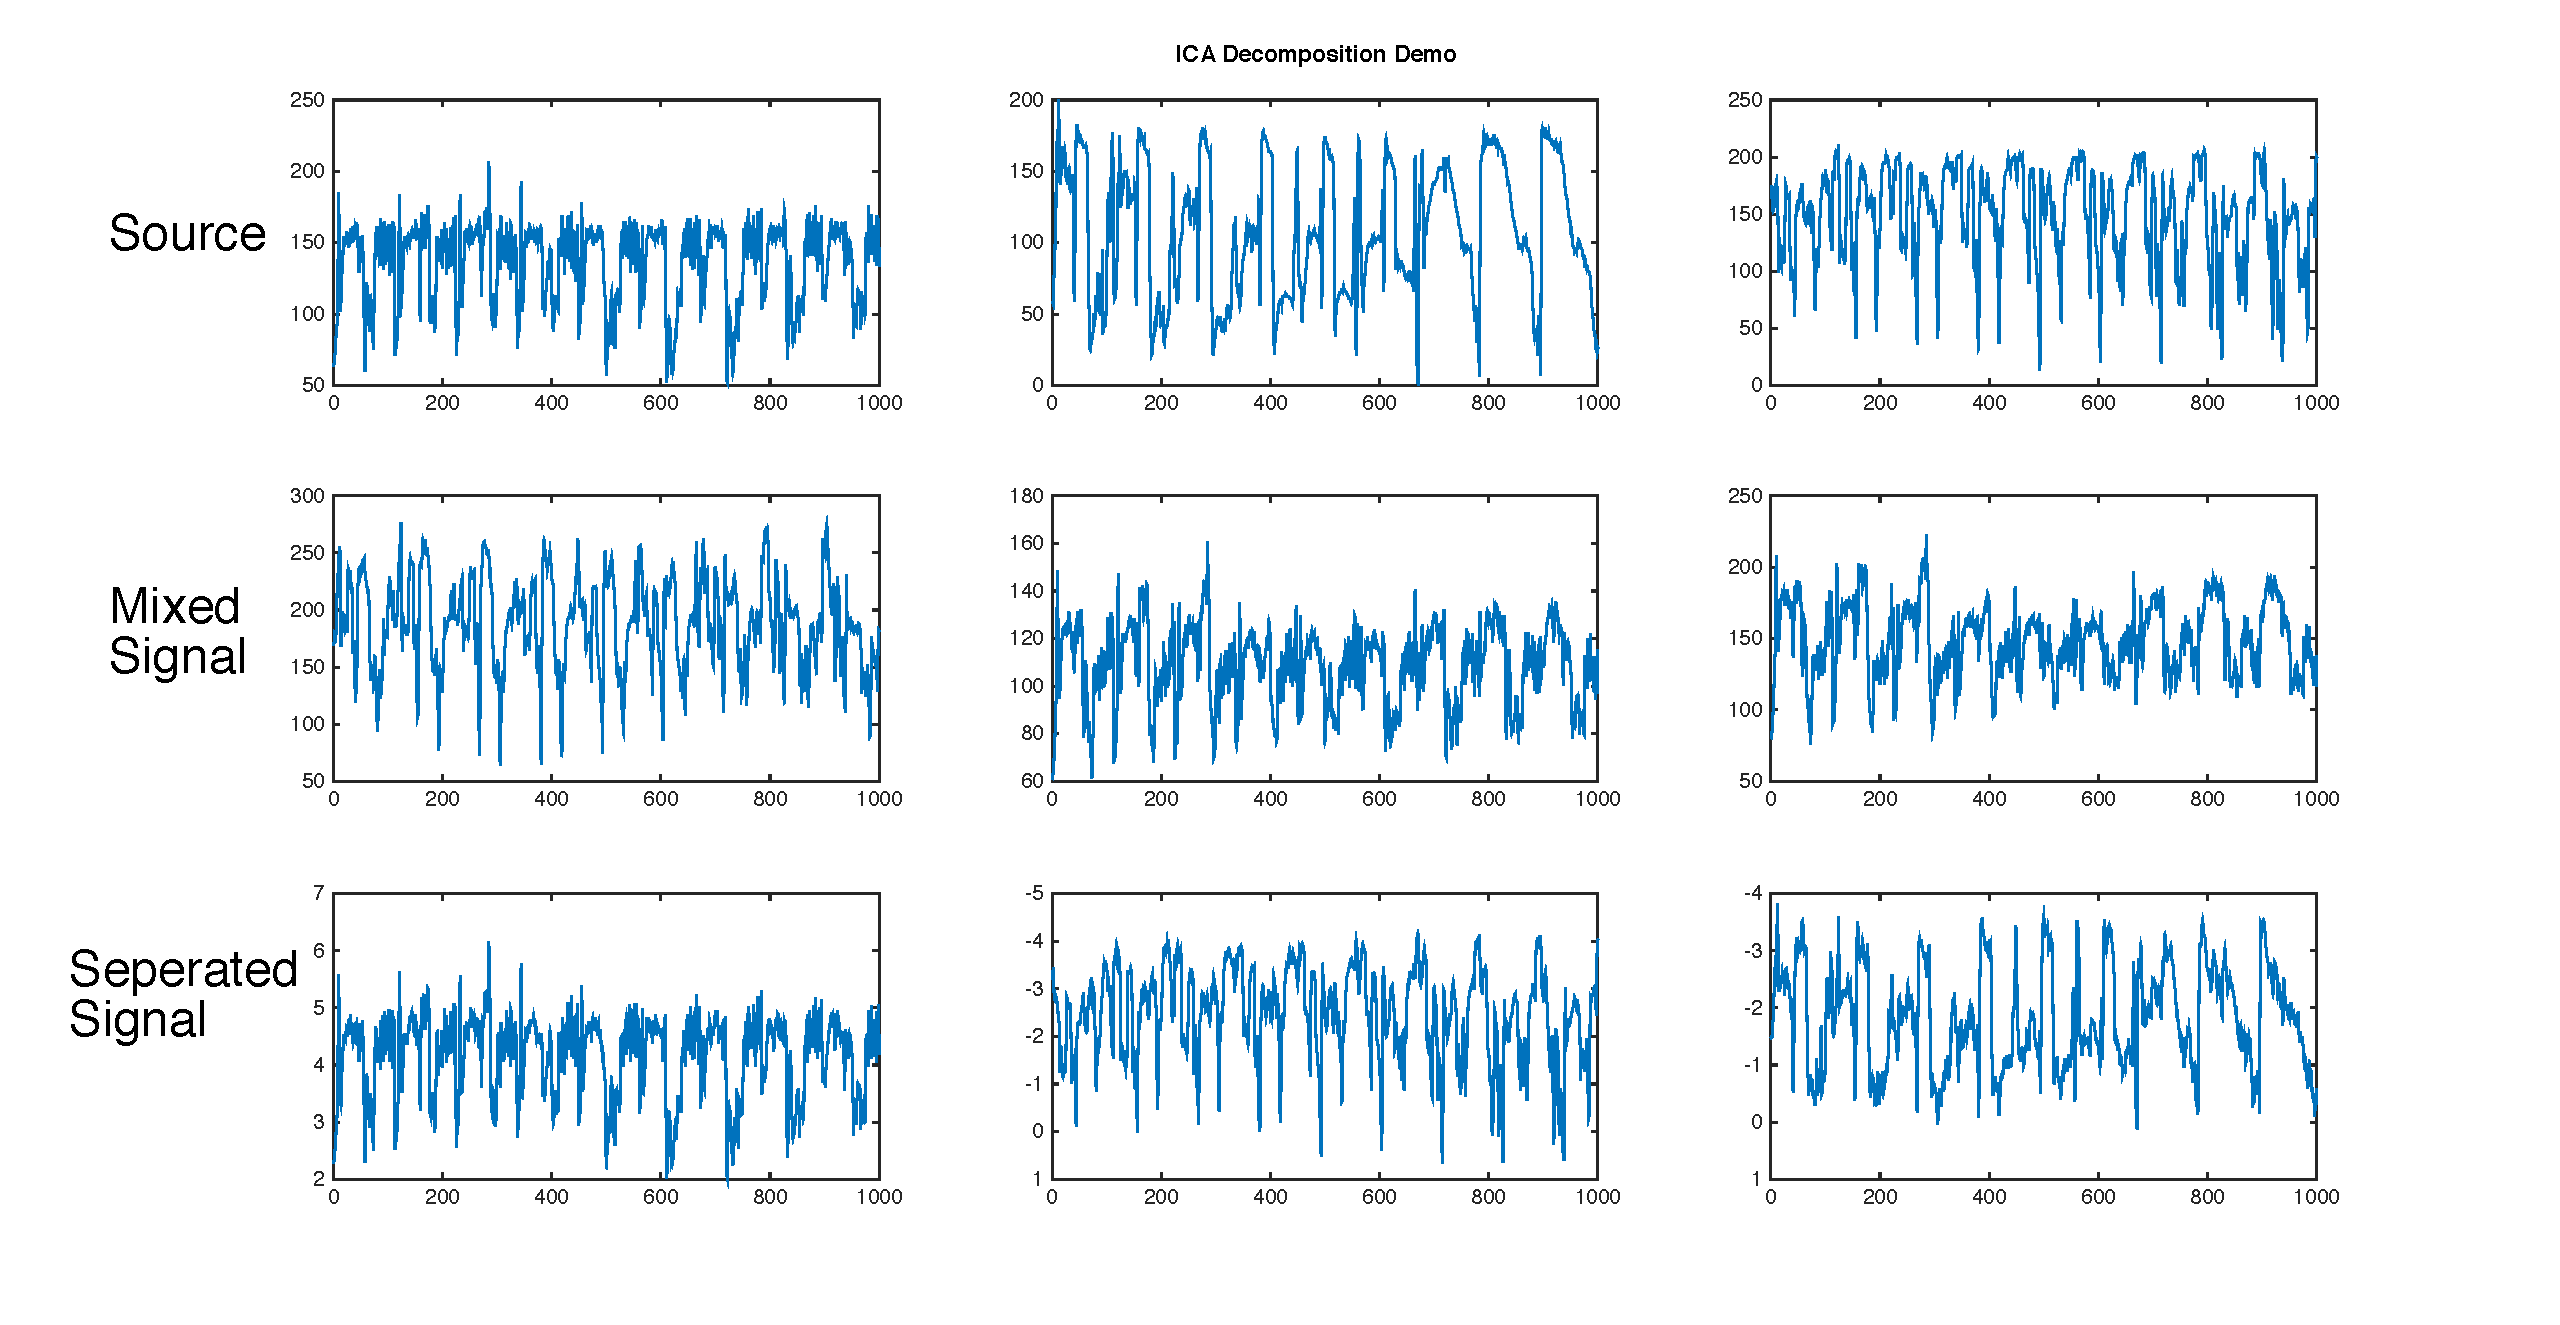
\includegraphics[width=\textwidth]{Img/ica_decom.pdf} 
\captionof{figure}{ICA解混示意\\ 由于ICA使相位改变了,解混信号被翻转了}
\label{fig:icadecom}
}
\end{minipage}
\medskip
\end{center}

可以明显看到,信号1和解混后信号1,信号2和解混后信号3,信号3和解混后信号2是比较相像的.说明ICA已经成功从第二栏的输入信号中分解出了原始信号.当然了,由于ICA作用于矩阵的缺点,解混信号的顺序,相位都被打乱了.
\paragraph{ICA作用于二维的变量}
实际了,上述3个长度1000的随机向量是3张$112 \times 92$图片的前1000元素,而ICA实际上也是作用于这3张混合后的图片的,以下是分解的结果:

\begin{center}
\begin{minipage}[t]{\linewidth}
\center
{
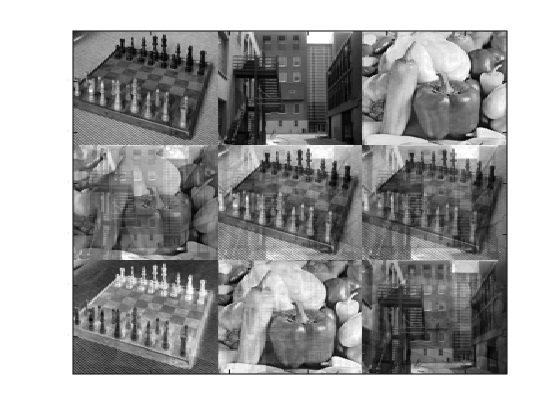
\includegraphics[width=\textwidth]{Img/ica_decom2.png} \captionof{figure}{2D ICA解混示意\\ 由于ICA使相位改变了,解混信号被翻转了}
	\label{fig:icadecom2}
}
\end{minipage}
\medskip
\end{center}
图片放置的顺序和\ref{fig:icadecom}一样,可见,ICA成功得从第二栏混合后的向量中分解出了第一栏的图片.\newline

从此就引出了ICA作用于人脸图像的动机了,如果输入人脸图像是\ref{fig:icadecom2}的第二栏图像,我们也用相同的方法来分解,必然能得到一些分解的结果.当假定人脸图像是有若干独立的变量线性组合而成的,自然地,我们就得到了第三栏这些分量.而这些分量具有相互独立的性质,本项目假定人脸图像就是由这些分量组合而来的,并以其作为投影的基底.


\subsection{ICA的在ORL测试集的投影基底}
以下是使用ORL数据集120张图片作为基底(40个人,每人三张),选择结果的前64张图片得到的特征基底.只选择120个图片用来计算是因为ICA的计算速度较慢.
\begin{center}
\begin{minipage}[t]{\linewidth}
%\label{fig:main}
\center
{
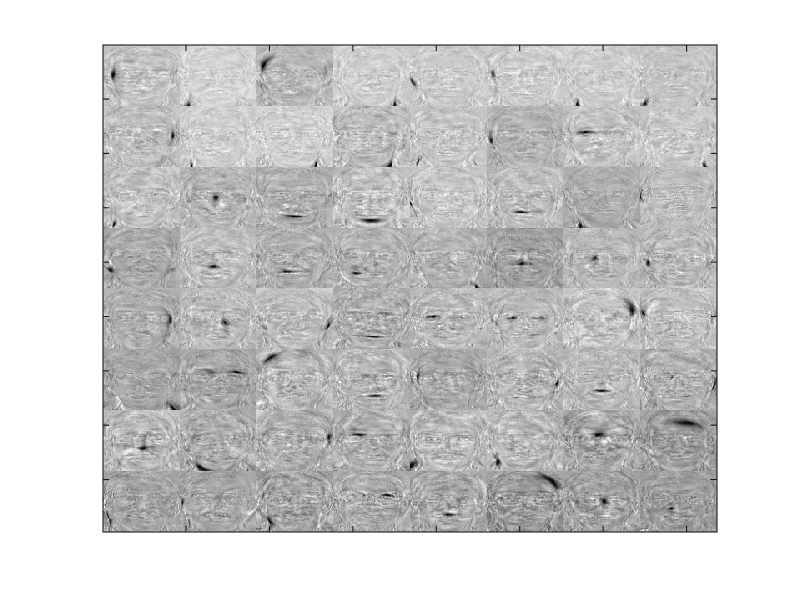
\includegraphics[width=\textwidth]{Img/ica_base.png} \captionof{figure}{ICA的在ORL测试集的投影基底}
\label{fig:ica_base}
}
\end{minipage}
\medskip
\end{center}
由于ICA基底不是正交的,使用了\textit{Matlab}函数中\textit{Pinv()}函数计算了伪逆来投影.



需要指出的是,ICA分解结果具有较强的稀疏性,因此也被用来压缩图像.这在\ref{fig:ica_base}中,可以看出大部分特征脸的部分都接近于0(近乎白色或者灰色)

%\section{DCT}
%在之前的实践中,笔者发现实际上任何图片的较为短小的并且与图片有较大联系的相关向量都可以被当做特征向量.这里,本项目从频域的角度出发,提取了图片的频域基频特征.
%\section{更多的基底}
%除了这些方法,还有很多其他的方法.\cite{de2010face}列出了更为详尽的列表,限于项目时间的限制,并没有深入研究这些所有的算法,仅仅尽可能的通过\textit{SciKit}工具包来列出相同测试样本下的基底.
%	\begin{itemize}
%		\item Kernel PCA
%		\item Weighted PCA
%		\item Linear Discriminant Analysis (LDA)
%		\item Kernel LDA
%		\item Semi-supervised Discriminant Analysis (SDA)
%		\item Neural Network based methods
%		\item Multidimensional Scaling (MDS)
%		\item Self-organizing map (SOM)
%		\item Active Shape Models (ASM)
%		\item Active Appearance Models (AAM)
%		\item Gavor wavelet transforms
%		\item MMSD, SMSD
%	\end{itemize}

\section{相关实验}
参见\ref{sec:comp_global}.




	